\def\nbrcircles {377}
\def\outerradius {30mm}
\def\deviation {.9}
\def\fudge {.62}

\newcounter{cumulArea}
\setcounter{cumulArea}{0}

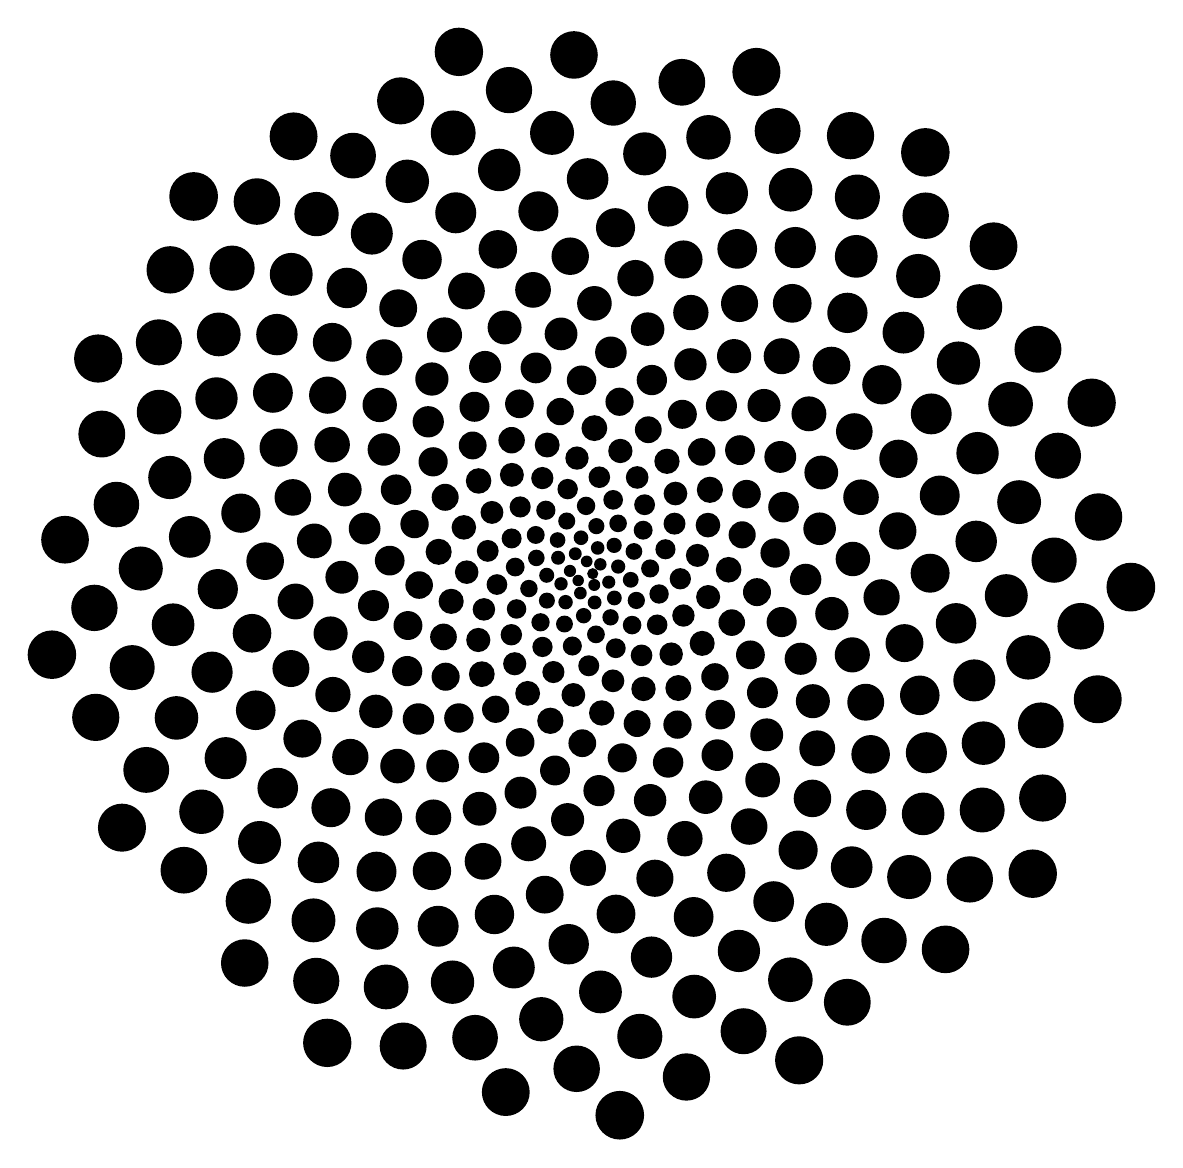
\begin{tikzpicture}[scale=.32]

\pgfmathsetmacro {\goldenRatio} {(1+sqrt(5))}
\pgfmathsetmacro {\meanArea}
      {pow(\outerradius * 10 / \nbrcircles, 2) * pi}
\pgfmathsetmacro {\minArea} {\meanArea * (1 - \deviation)}
\pgfmathsetmacro {\midArea} {\meanArea * (1 + \deviation) - \minArea}

\foreach \b in {0,...,\nbrcircles}{
    % mod() must be used in order to calculate the right angle.
    % otherwise, when \b is greater than 28 the angle is greater
    % than 16384 and an error is raised ('Dimension too large').
    % -- thx Tonio for this one.
    \pgfmathsetmacro{\angle}{mod(\goldenRatio * \b, 2) * 180}

    \pgfmathsetmacro{\sratio}{\b / \nbrcircles}
    \pgfmathsetmacro{\smArea}{\minArea + \sratio * \midArea}
    \pgfmathsetmacro{\smRadius}{sqrt(\smArea / pi) / 2 * \fudge}
    \addtocounter{cumulArea}{\smArea};

    \pgfmathparse{sqrt(\value{cumulArea} / pi) / 2}
    \fill[] (\angle:\pgfmathresult) circle [radius=\smRadius] ;
}  
\end{tikzpicture}
